% \iffalse meta-comment --------------------------------------------------
% Copyright (C) 2021 SJTUG
%
% Licensed under the Apache License, Version 2.0 (the "License");
% you may not use this file except in compliance with the License.
% You may obtain a copy of the License at
%
%     http://www.apache.org/licenses/LICENSE-2.0
%
% Unless required by applicable law or agreed to in writing, software 
% distributed under the License is distributed on an "AS IS" BASIS,
% WITHOUT WARRANTIES OR CONDITIONS OF ANY KIND, either express or implied.
% See the License for the specific language governing permissions and
% limitations under the License.
% ------------------------------------------------------------------------ \fi
% \iffalse
%<*package>
\NeedsTeXFormat{LaTeX2e}
\ProvidesPackage{beamerinnerthemesjtubeamer}[2021/11/22 sjtubeamer inner theme v2.3.1]
%</package>
% \fi
% \CheckSum{0}
% \StopEventually{}
% \iffalse
%<*package>
% ------------------------------------------------------------------- \fi
%
%
% \subsection{Inner Theme}
%
%
% A |beamer| inner theme dictates the style of the frame elements traditionally
% set in the ``body'' of each slide. These include:
%
% \begin{itemize}
%   \item title, part, and section pages;
%   \item itemize, enumerate, and description environments;
%   \item block environments including theorems and proofs;
%   \item figures and tables; and
%   \item footnotes and plain text.
% \end{itemize}
%
%  \subsubsection{Load Packages}
%   Load SJTU VI Library to get the definition on color and shape.
%    \begin{macrocode}
\RequirePackage{sjtuvi}
%    \end{macrocode}
%   Load tcolorbox for creating delicate boxes.
%    \begin{macrocode}
\RequirePackage{tcolorbox}
%    \end{macrocode}
%
%   \subsubsection{Option Declaration}
%  \begin{macro}{\sjtubeamer@inner@cover}
%    \begin{macrocode}
%<*maxplus>
\DeclareOptionBeamer{maxplus}{\def\sjtubeamer@inner@cover{maxplus}}
%</maxplus>
%<*max>
\DeclareOptionBeamer{max}{\def\sjtubeamer@inner@cover{max}}
%</max>
%<*min>
\DeclareOptionBeamer{min}{\def\sjtubeamer@inner@cover{min}}
%</min>
%<*my>
\DeclareOptionBeamer{my}{\def\sjtubeamer@inner@cover{my}} % reserved for customization
%</my>
\ExecuteOptionsBeamer{
%<*maxplus>
  maxplus,
%</maxplus>
%<*min>
  min,
%</min>
%<*my>
  my,
%</my>    
%<*max>
  max,
%</max>
}
%    \end{macrocode}
%  \end{macro}
%
%  \begin{macro}{\sjtubeamer@inner@lang}
%    \begin{macrocode}
\DefineOption{inner}{lang}{cn}
\DefineOption{inner}{lang}{en}
\@ifclassloaded{ctexbeamer}{\ExecuteOptionsBeamer{cn}}{
  \ExecuteOptionsBeamer{en}}
%    \end{macrocode}
%  \end{macro}
%
%  \begin{macro}{\sjtubeamer@inner@color}
%    \begin{macrocode}
\DefineOption{inner}{color}{red}
\DefineOption{inner}{color}{blue}
\ExecuteOptionsBeamer{red}
%    \end{macrocode}
%  \end{macro}
%
%    \begin{macrocode}
\ProcessOptionsBeamer
\PassOptionsToPackage{\sjtubeamer@inner@cover}{sjtucover}
%    \end{macrocode}
%
%   Hard-coded color for blocks. A replica of color theme.
%    \begin{macrocode}
\if\EqualOption{inner}{color}{red}
  \colorlet{cprimary}{sjtuRedPrimary}
  \colorlet{csecondary}{sjtuRedSecondary}
  \colorlet{ctertiary}{sjtuRedTertiary}
  \colorlet{cquanternary}{black}
\else
  \colorlet{cprimary}{sjtuBluePrimary}
  \colorlet{csecondary}{sjtuBlueSecondary}
  \colorlet{ctertiary}{sjtuBlueTertiary}
  \colorlet{cquanternary}{white}
\fi
%    \end{macrocode}
%
%  \begin{macro}{\sjtubeamer@logocolor}
%   Change the color variable that controls the logo color to current main color of this theme. Since this template doesn't design a dark background for the contents (it is really not easy to handle with the contents for a dark background).
%    \begin{macrocode}
\def\sjtubeamer@logocolor{cprimary}
%    \end{macrocode}
%  \end{macro}
%
%   \subsubsection{Load Packages}
%
%   Introduce the library from tcolorbox to make code blocks.
%   \verb"listingsutf8" is used to receive UTF-8 input. 
%   The global set on shield externalize will prevent tcolorbox from externalizing. 
%    \begin{macrocode}
\RequirePackage{tcolorbox}
\tcbuselibrary{skins}
\tcbuselibrary{listingsutf8}
\tcbset{shield externalize}
%    \end{macrocode}
%
% \subsubsection{Title Page \& Bottom Page}
%
%  \begin{macro}{\logo}
%  Define logo.
%    \begin{macrocode}
\usebeamercolor{palette primary}
%<*max>
\if\EqualOption{inner}{cover}{max}
  \logo{\resizebox{!}{1cm}{\sjtubadge}}
\else
%</max>
  \if\EqualOption{inner}{lang}{cn}
    \logo{\resizebox{!}{0.7cm}{\cnlogo}}
  \else
    \logo{\resizebox{!}{0.7cm}{\enlogo}}
  \fi
%<*max>
\fi
%</max>
%    \end{macrocode}
%  \end{macro}
%
%  \begin{macro}{\bgcenterbox}
%   Define a command for USERS to make a centered background box easily. Move the defination on \verb"\sjtubeamer@logocolor" to the inner environment, to avoid the shift on centering. And since the definition has already been moved into the inner group, the definition here is \emph{locale} and no more stack saving is needed.
%    \begin{macrocode}
\newcommand{\bgcenterbox}[1]{
  \parbox[c][1.1\paperheight][c]{\paperwidth}{
    \def\sjtubeamer@logocolor{cprimary!50}
    \centering\resizebox{\paperwidth}{!}{#1}
  }
}
%    \end{macrocode}
%  \end{macro}
%
%  \begin{macro}{\titlegraphic}
% Define the title grahic image.
%
% NOTICE: if you are using your own title graphic, please use png image with predefined color and transparency. Since it is beyond the control of logo color system. Or you could use the provided command in the sjtuvi library to create your own masked picture in order to follow the logo color system (The provided picture should be white and transparent in the background).
%
%    max theme has the background.
%    \begin{macrocode}
%<*maxplus>
\if\EqualOption{inner}{cover}{maxplus}
  \titlegraphic{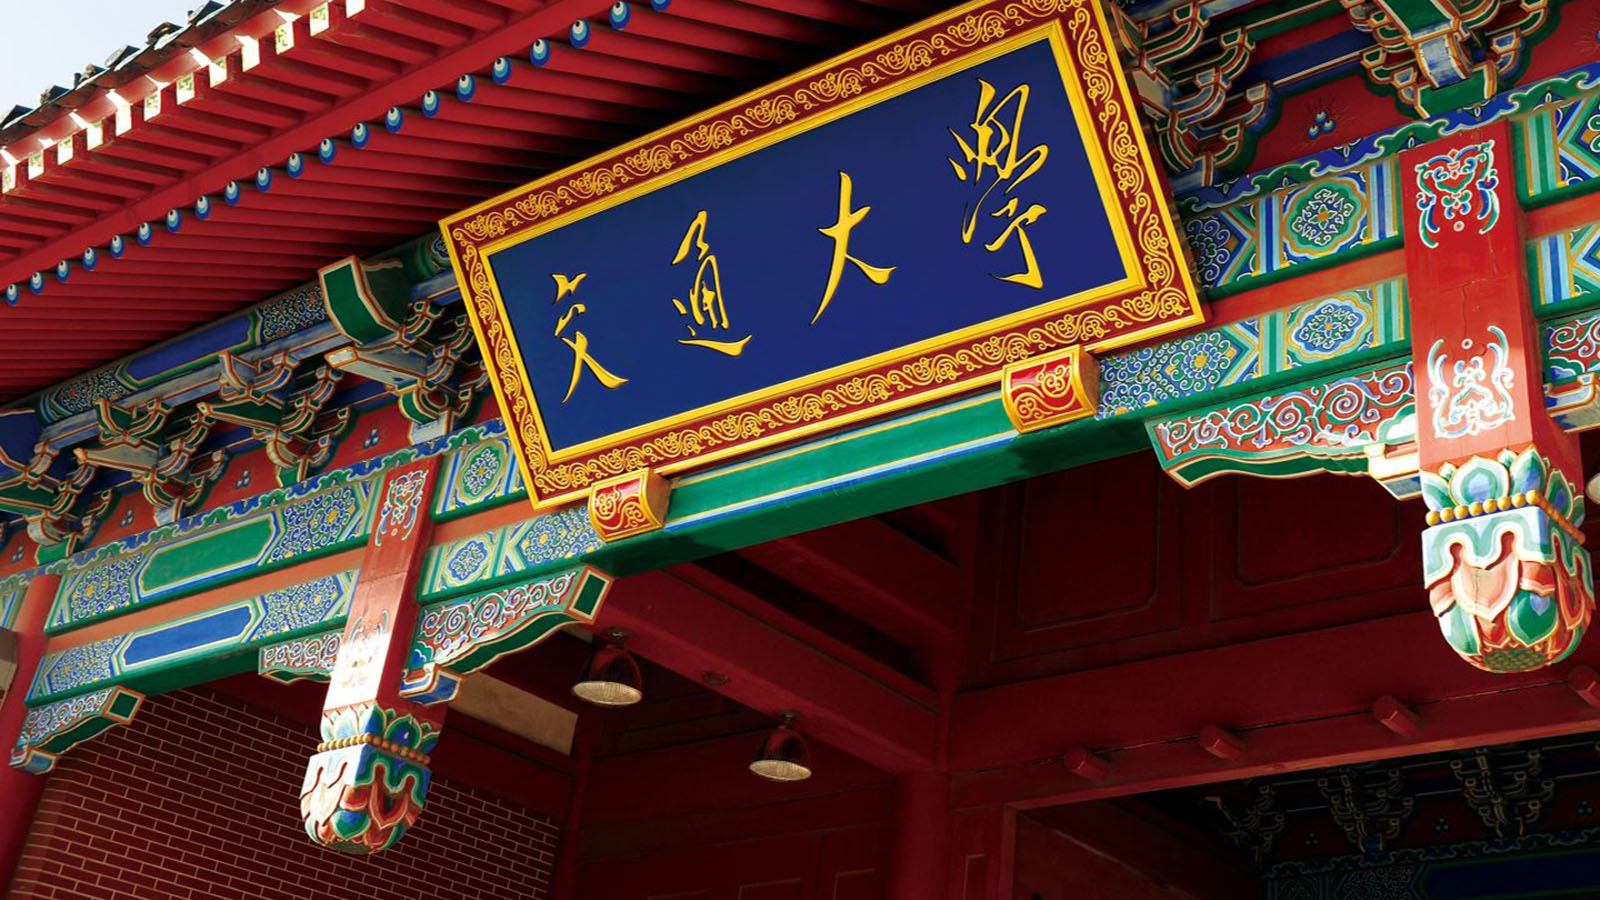
\includegraphics{vi/sjtuphoto.jpg}}
\else
%</maxplus>
%<*max>
  \if\EqualOption{inner}{cover}{max}
    \usebeamercolor{palatte primary}
    \titlegraphic{\sjtubg[opacity=0.2]}
    \setbeamertemplate{background}
    {\bgcenterbox{\sjtubg[cprimary!50,opacity=0.2]}}
  \else
%</max>
%<*min>
    \if\EqualOption{inner}{cover}{min}
      \titlegraphic{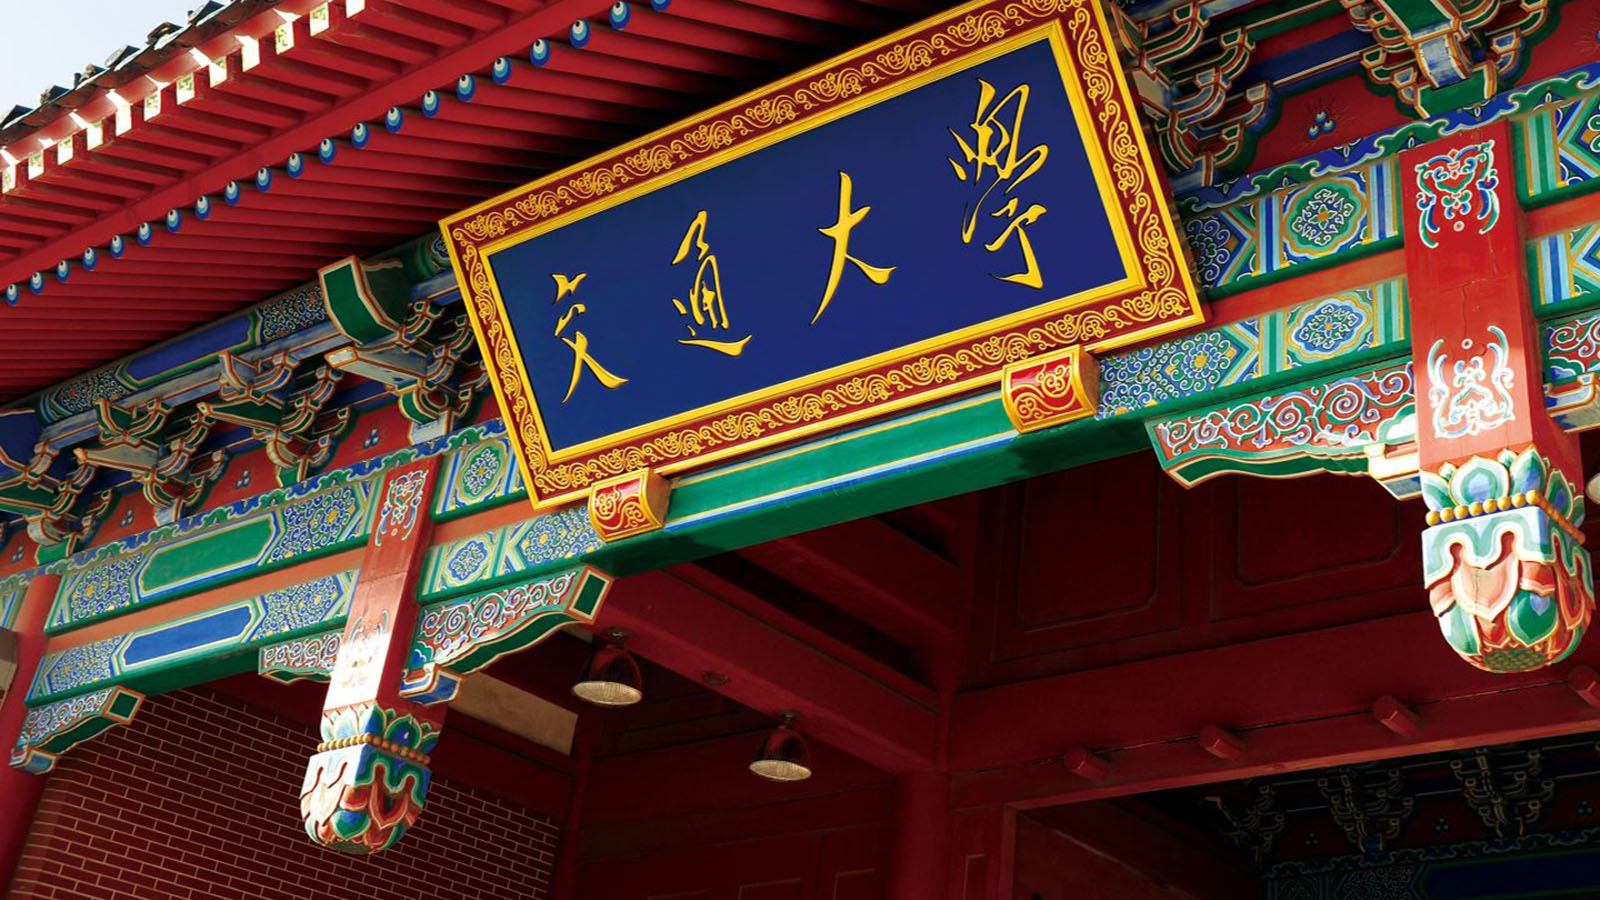
\includegraphics{vi/sjtuphoto.jpg}}
    \else
%</min>
%<*my>
      \if\EqualOption{inner}{cover}{my}
        %
        % Developer could define your title graphic here for "my"...
        %
        \titlegraphic{}
      \else
%</my>
%<*my>
      \fi
%</my>
%<*min>
    \fi
%</min>
%<*max>
  \fi
%</max>
%<*maxplus>
\fi
%</maxplus>
%    \end{macrocode}
%  \end{macro}
%
%
%  Initialize sidebar width to 0pt as no sidebar required, which will be overwritten in outer theme.
%    \begin{macrocode}
\newdimen\beamer@sidebarwidth
\beamer@sidebarwidth=0pt
%    \end{macrocode}
%
%  \begin{macro}{\coverpage}
%  Common command for \verb"\titlepage" and \verb"\bottompage". Disable externalization for generating title page and bottom page, locally.
%  Since the definition on \verb"\sjtubeamer@logocolor" is defined in a group, the stack is not necessary to store the value.
%    \begin{macrocode}
\def\coverpage#1{
  {
    \tikzset{external/export=false}
    \ifdim\beamer@sidebarwidth=0pt %
      \usebeamertemplate*{#1}
    \else
      \hspace*{-0.5\beamer@sidebarwidth}\parbox[t]{\textwidth}{
        \usebeamertemplate*{#1}
      }
    \fi
  }
}
%    \end{macrocode}
%  \end{macro}
%
%  \begin{macro}{\titlepage}
%   Call the title page template to make a title page. This is a patch for the original \verb"\titlepage" command, to fit with the logo color system.
%    \begin{macrocode}
\def\titlepage{
  \coverpage{title page}
}
%    \end{macrocode}
%  \end{macro}
%
%  \begin{macro}{\maketitle}
%  Patch make title command. It will receive an optional argument for switching different type of title page. The set on beamer template is inside a group, so the setting is locale.
%    \begin{macrocode}
\renewcommand{\maketitle}[1][\sjtubeamer@inner@cover]{
  {
    \setbeamertemplate{title page}[#1]
    \ifbeamer@inframe\titlepage\else
      \begin{frame}[plain]
        \titlepage
      \end{frame}\fi
  }
}
%    \end{macrocode}
%  \end{macro}
%
%  \begin{macro}{\bottompage}
%   Call the bottom page template to make a bottom page.
%    \begin{macrocode}
\def\bottompage{
  \coverpage{bottom page}
}
%    \end{macrocode}
%  \end{macro}
%
%  \begin{macro}{\bottomthanks}
%  The "Thank You" caption in the bottom page.
%    \begin{macrocode}
\if\EqualOption{inner}{lang}{cn}%
  \def\bottomthanks{谢\,谢}
\else%
  \def\bottomthanks{Thank You}
\fi%
%    \end{macrocode}
%  \end{macro}
%
%  \begin{macro}{\makebottom}
%   Make the bottom page. Not a built-in command.
%   Redefinition on \verb"\beamer@writeslideentrty" locally will remove the corresponding navigation dot for miniframe outer theme. This is not necessary for title page, since it should not belong to any sections.
%    \begin{macrocode}
\newcommand{\makebottom}[1][\sjtubeamer@inner@cover]{
  {
    \def\beamer@writeslidentry{\clearpage\beamer@notesactions}
    \setbeamertemplate{bottom page}[#1][\bottomthanks]
    \ifbeamer@inframe\bottompage\else
      \begin{frame}[plain]
        \bottompage
      \end{frame}\fi
  }
}
%    \end{macrocode}
%  \end{macro}
%
%   Load Cover Library to get the customized cover.
%    \begin{macrocode}
\RequirePackage{sjtucover}
%    \end{macrocode}
%
% \subsubsection{Part Page}
%  \begin{macro}{\partpage}
%   Define the \verb"part page" beamer template.
%    \begin{macrocode}
\defbeamertemplate*{part page}{sjtubeamer}[1][]
{
  \vfill
  \vskip 8pt
  \begingroup
%    \end{macrocode}
%   Print the number of this part. If it is in Chinese, the translated version is printed.
%    \begin{macrocode}
  \begin{beamercolorbox}[sep=16pt,right,#1]{part title}
    \hfill\usebeamerfont{part name}
    \if\EqualOption{inner}{lang}{cn}%
    第~\insertromanpartnumber~部分
    \else%
    \partname~\insertromanpartnumber
    \fi%
    \par\vskip4pt
    \usebeamerfont{part title}\insertpart\par
%    \end{macrocode}
%   Since navigation bar is packaged, to modify the color, you have to change the \verb"section in head/foot" beamer color. Here, the first move is to save the current color to a temporary variable. After the insertion, the previous color should be restored.
%    \begin{macrocode}
    \hbox to \textwidth{
      \usebeamerfont{footline}%
      \setbeamercolor{tempcolor}{fg=section in head/foot.fg}
      \setbeamercolor{section in head/foot}{use=palette primary,
        fg=palette primary.fg,bg=}
      \hfill
      \insertnavigation{0.4\textwidth}
      \hspace*{1cm}
      \setbeamercolor{section in head/foot}{fg=tempcolor.fg}
    }
  \end{beamercolorbox}
  \endgroup
  \vfill
}
%    \end{macrocode}
%  \end{macro}
%
%  \begin{macro}{\part}
%   Redirect the part command to make a part page.
%   Redefinition on \verb"\beamer@writeslideentrty" locally will remove the corresponding navigation dot like what it has been done in the bottom page.
%    \begin{macrocode}
\AtBeginPart{
  {
    \def\beamer@writeslidentry{\clearpage\beamer@notesactions}
    \begin{frame}[plain]
      \partpage
    \end{frame}
  }
}
%    \end{macrocode}
%  \end{macro}
%
% \subsubsection{Section Page \& Subsection Page}
%   Define the common \verb"\sectionblock" command to make the section block.
%    \begin{macrocode}
\def\sectionblock#1{
  \begin{beamercolorbox}[sep=12pt,right,#1]{section title}
    \usebeamerfont{section name}
    \if\EqualOption{inner}{lang}{cn}%
    第~\insertsectionnumber~节
    \else%
    \sectionname~\insertsectionnumber
    \fi%
    \par\vskip4pt
    \usebeamerfont{section title}\insertsection\par
  \end{beamercolorbox}
}
%    \end{macrocode}
%
%  \begin{macro}{\sectionpage}
%   Define the \verb"section page" beamer template.
%    \begin{macrocode}
\defbeamertemplate*{section page}{sjtubeamer}[1][]
{
  \vfill
  \begingroup
  \sectionblock{#1}
  \endgroup
  \vfill
}
%    \end{macrocode}
%  \end{macro}
%
%  \begin{macro}{\subsectionpage}
%   Define the \verb"subection page" beamer template.
%    \begin{macrocode}
\defbeamertemplate*{subsection page}{sjtubeamer}[1][]
{
  \vfill
  \begingroup
  \sectionblock{#1}
  \begin{beamercolorbox}[sep=8pt,right,#1]{subsection title}
    \usebeamerfont{subsection name}
    \if\EqualOption{inner}{lang}{cn}%
    第~\insertsubsectionnumber~小节
    \else%
    \subsectionname~\insertsubsectionnumber
    \fi%
    \par\vskip 4pt
    \usebeamerfont{subsection title}\insertsubsection\par
  \end{beamercolorbox}
  \endgroup
  \vfill
}
%    \end{macrocode}
%  \end{macro}
%
% \subsubsection{Itemize Environments}
%
%   Set the item marker to circle and set the marker for section and subsection in TOC (Table of Contents) to circle.
%    \begin{macrocode}
\useinnertheme{circles}
%    \end{macrocode}
%
% \subsubsection{Block Environments}
%
%   The block in \verb"min" theme is not rounded.
%    \begin{macrocode}
%<*min>
\if\EqualOption{inner}{cover}{min}\else
%</min>
  \setbeamertemplate{blocks}[rounded]
%<*min>
\fi
%</min>
%    \end{macrocode}
%
% \begin{macro}{\highlight}
%   Highlight the given text. Create a primary color background block with white as foreground.
%    \begin{macrocode}
\newtcbox{\highlight}[1][cprimary]{
  on line,
  arc=0pt,
  colback=#1,
  colupper=white,
  boxrule=0pt,
  boxsep=0pt,
  left=4pt,
  right=4pt,
  top=2pt,
  bottom=2pt
}
%    \end{macrocode}
% \end{macro}
%
% \begin{macro}{\paragraph}
%   Use \verb"\highlight" macro for making contrast.
%   Since beamer has deleted \verb"\paragraph" macro in this class, this template defines a macro for that to indicate it is another point and more paragraph-like. It is useful for the migration from \verb"article" class.
%    \begin{macrocode}
\providecommand{\paragraph}[1]{
  \highlight{#1}~
}
%    \end{macrocode}
% \end{macro}
%
% \begin{macro}{stampbox}
%   Make a stampbox border, which is a decoration advice from SJTU VI. It has the dependency on \verb"stampline" from \verb"sjtuvi" package.
%    \begin{macrocode}
\newtcolorbox{stampbox}[1][cprimary]{%
  capture=hbox,
  enhanced,
  frame empty,
  interior empty,
  sharp corners,
  top=2pt,bottom=2pt,left=2pt,right=2pt,
  borderline={4pt}{0pt}{
    #1,
    line width=0.5pt,
    decoration={
      stampline,
      segment length=8pt,
      path has corners=true,
    },
    decorate
  }
}
%    \end{macrocode}
% \end{macro}
%
%   Declare the basic listing highlighter. \verb"columns" is set to \verb"flexible" to avoid ugly grid alignment. \verb"breaklines" is set to enable line wrapping.
%    \begin{macrocode}
\lstset{
  basicstyle=\ttfamily\small,
  keywordstyle=\color{cprimary},%
  stringstyle=\color{csecondary},%
  commentstyle=\color{ctertiary!80!gray},%
  columns=flexible,
  extendedchars=false,
  showstringspaces=false,
  showspaces=false,
  breaklines
}
%    \end{macrocode}
%
% \begin{macro}{codeblock}
%   Code block environment is made for presenting code in an obvious way. Two parameters are required. The first parameter is passed to listing, which mostly sets the language to highlight, see the \verb"listings" package for more details. And the second parameter receives the title to make.
%    \begin{macrocode}
\newtcblisting{codeblock}[2][]{
  listing only,
  listing engine=listings,
  listing options={
    #1,%
    numbers=left,
    numberstyle=\color{cprimary!80}\ttfamily\scriptsize,
    numbersep=5pt,
  },
  enhanced,
  sharp corners,
  top=0mm,
  bottom=0mm,
  title=#2,
  colback=cprimary!5,
  colframe=cprimary!80,
  overlay={
    \begin{tcbclipinterior}\fill[cprimary!20]%
      (frame.south west) rectangle ([xshift=5mm]frame.north west);
    \end{tcbclipinterior}
  }
}
%    \end{macrocode}
% \end{macro}
%
%   Extra Support for pgfplots and pgfplotstable (if loaded in the main file).
%    \begin{macrocode}
\AtEndPreamble{%
%    \end{macrocode}
%   Set the default visual theme for \textsc{Pgfplots}. The cycle list is set to the current color theme. And lines on the graph is optimized to make it clear for presentation. The predefinition on the height is made to avoid the overfullbox on the vertical side.
%    \begin{macrocode}
  \@ifpackageloaded{pgfplots}{%
    \pgfplotsset{
      compat=newest,
      every axis/.style={
        font=\small\sffamily,
        cycle multi list={
            mark options={thick}\nextlist
            mark list\nextlist
            cprimary,csecondary,ctertiary\nextlist
          },
        height=0.5*\the\paperheight,
        axis line style={
            cprimary,
            thin
          },
        every tick label/.style={
            cprimary,
            font=\small,
            /pgf/number format/assume math mode=true
          },
        grid style={cprimary!10},
        tick style={cprimary!50},
        minor tick style={cprimary!30},
        xlabel style={cprimary},
        ylabel style={cprimary},
        zlabel style={cprimary},
        legend style={
            draw={cprimary},
            thin,
            nodes={cprimary}
          },
        thick,
      },
    }
  }{}
%    \end{macrocode}
%   Set the style of \textsc{Pgfplotstable}. The \verb"\colorrows" macro here is used for making the header colored. The \verb"booktabs" line is used to create a professional look.
%    \begin{macrocode}
  \@ifpackageloaded{pgfplotstable}{%
    \RequirePackage{array}
    \RequirePackage{colortbl}
    \RequirePackage{booktabs}
%    \end{macrocode}
%   Two macros are defined to make the header colored.
%    \begin{macrocode}
    \def\zapcolorreset{\let\reset@color\relax\ignorespaces}
    \def\colorrows#1{\noalign{\aftergroup\zapcolorreset#1}\ignorespaces}
%    \end{macrocode}
%    \begin{macrocode}
    \pgfplotstableset{
      col sep=comma,
      every table/.style={
        font={\small\sffamily},
      },
      every head row/.style={
        before row={
          \arrayrulecolor{cprimary}
          \toprule
          \colorrows{\color{cprimary}}
        },
        after row={
            \midrule
            \colorrows{\color{black}}
          },
        },
      every last row/.style={
        after row=\bottomrule
      },
    }
    \newcolumntype{L}[1]{>{\begin{pgfplotstablecoltype}[#1]}
            r<{\end{pgfplotstablecoltype}}}
  }{}
%    \end{macrocode}
% Disable the warning from \verb"hyperref" which conflicts the setting in C\TeX{} or CJK. It has to be manually disabled.
%    \begin{macrocode}
  \def\Hy@WarnOptionDisabled#1{
    \def\next{#1}%
    \ifx\next pdfauthor %
      \ifx\next driverfallback %
      \else
        \Hy@Warning{%
          Option `#1' has already been used,\MessageBreak
          setting the option has no effect%
        }
      \fi%
    \fi%
  }
}
%    \end{macrocode}
%
% \iffalse
%</package>
% \fi
%
% \Finale
\endinput
